\documentclass[tikz,border=5pt,10pt]{standalone}
\usepackage{tikz}
\usetikzlibrary{calc}
\usepackage{pgf,xcolor}
\usepackage{eulervm}
\usepackage{booktabs,rotating,multirow,caption}
\usepackage{makecell}
\usetikzlibrary{automata}
\usetikzlibrary{arrows}
\usepackage{mathdots}
\usetikzlibrary{decorations.pathreplacing}
\usetikzlibrary{backgrounds}
\begin{document}
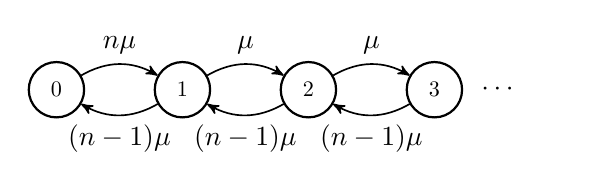
\begin{tikzpicture}[->, >=stealth', auto, semithick, node distance=2cm]
    \tikzstyle{every state}=[fill=white,draw=black,thick,text=black,scale=0.8]
    \node[state]    (0)				{$0$};
    \node[state]    (1)[right of=0]	{$1$};
    \node[state]    (2)[right of=1]	{$2$};
    \node[state]    (3)[right of=2]	{$3$};
    \node[state, draw=none]    (4)[right of=3]	{$ $};
    \path
    (0)
      edge[bend left]	node[above]{$n\mu$} 	(1)
    (1)
      edge[bend left] 	node[below]{$(n-1)\mu$}	(0)
      edge[bend left] 	node[above]{$\mu$}		(2)
    (2)
      edge[bend left]	node[below]{$(n-1)\mu$}	(1)
      edge[bend left]	node[above]{$\mu$}		(3)
    (3)
      edge[bend left]  node[below]{$(n-1)\mu$}	(2)
      edge[draw=none]	node[auto=false]{$\cdots$}	(4);
  \end{tikzpicture}
  \end{document}